\section{A machine model for programmable state manipulation on high-speed routers}
\label{s:absmachine}
\begin{figure}[!t]
  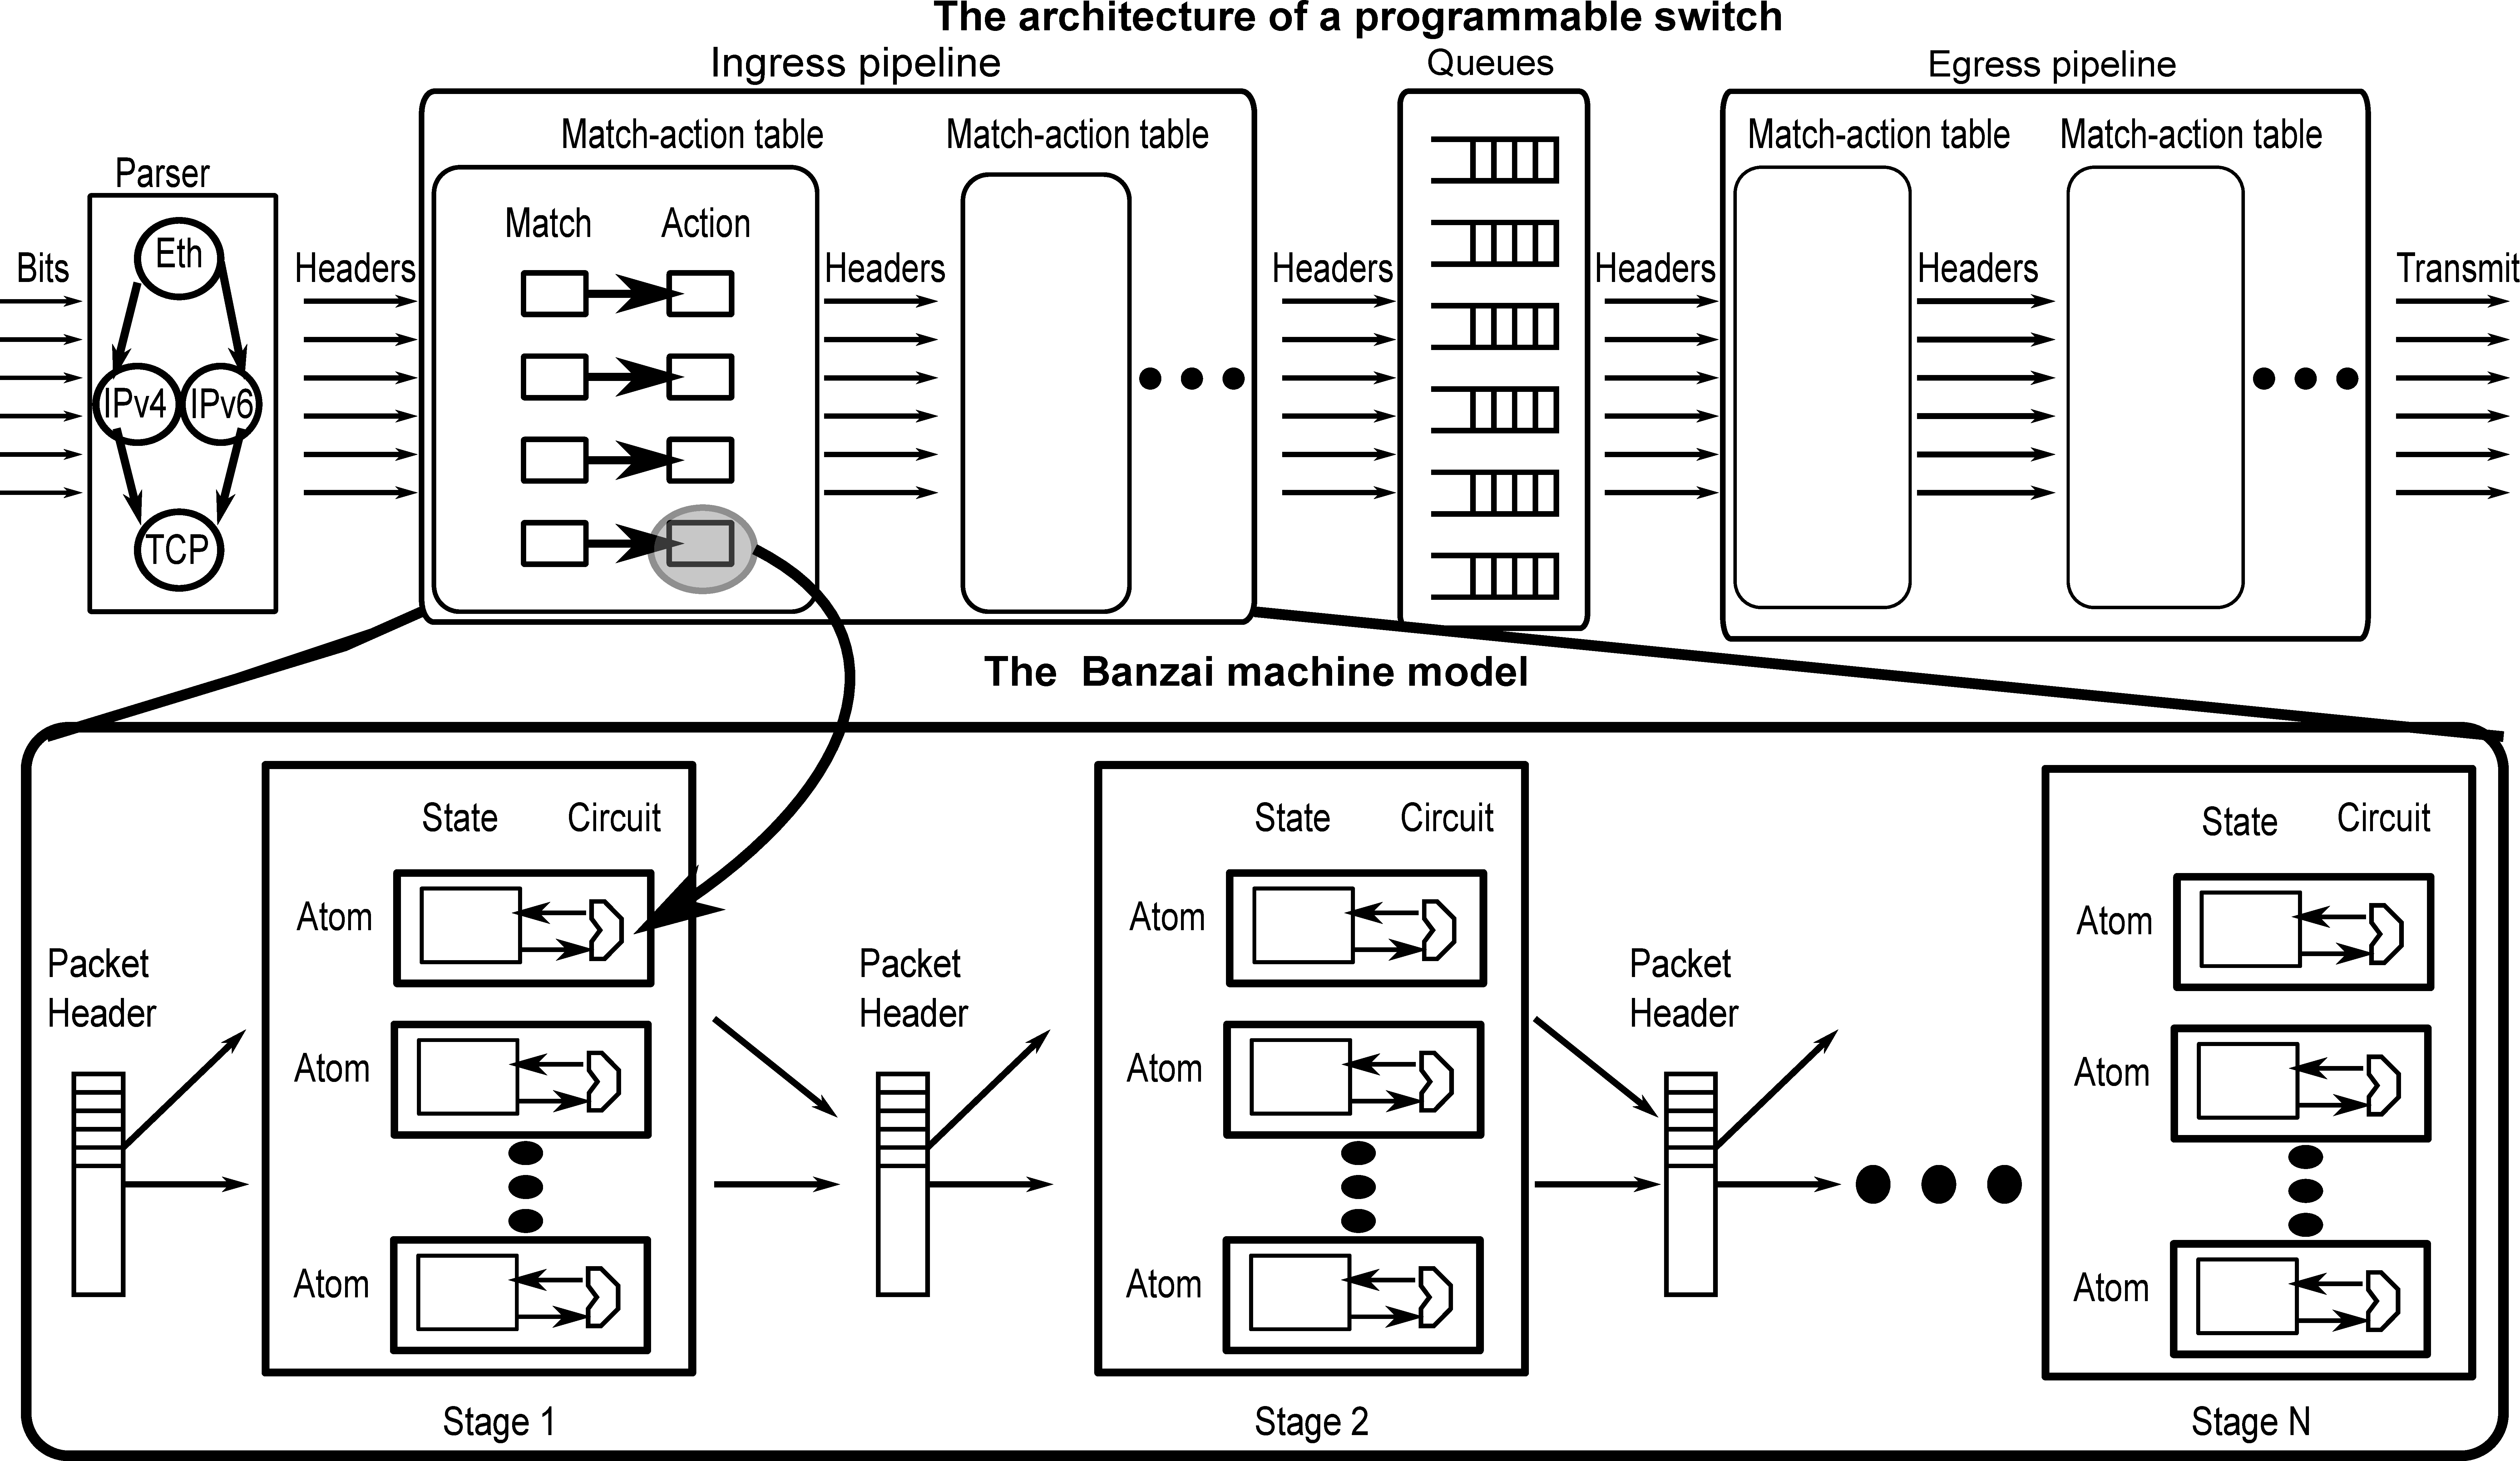
\includegraphics[width=\textwidth]{domino_banzai.pdf}
  \caption{\absmachine models the ingress or egress pipeline of a
  programmable router. An atom corresponds to an action in a match-action
  table. Internally, an atom contains local state and a digital circuit 
  modifying this state. Figure~\ref{fig:atom} details an atom.}
  \label{domino_fig:router}
\end{figure}

\absmachine is a machine model for programmable high-speed routers that serves
as the compiler target for \pktlanguage.  \absmachine is inspired by recent
programmable router architectures such as Barefoot Networks'
Tofino~\cite{tofino}, Intel's FlexPipe~\cite{flexpipe}, and Cavium's XPliant
Packet Architecture~\cite{xpliant}. \absmachine abstracts these architectures
and extends them with stateful processing units to implement data-plane
algorithms.  These processing units, called {\em atoms}, model atomic
operations that are supported by a programmable high-speed router. In other
words, atoms serve as the instruction set of the router.

Recall from Chapter~\ref{chap:arch} that high-speed routers are architected in
hardware as a pipeline where each pipeline stage processes a new packet every
clock cycle of 1 ns.  Having to process a packet every clock cycle in each
stage constrains the operations that can be performed on each packet. In
particular, any packet operation that modifies state visible to the next packet
is constrained to finish execution in a single clock cycle (\S\ref{ss:atoms}
shows why). Any programmable router chip will provide a small set of processing
units or primitives that respect these constraints. These primitives could be
used for manipulating packets and/or state in a stage and determine which
algorithms can or cannot run on the router. We now describe this concept of
constrained computation in greater detail.

%TODO: We talk about how to represent atoms and then again talk about constraining
% them using atom templates. They both represent atoms, so it's a bit confusing.

\begin{figure}[!t]
  \begin{subfigure}{0.5\columnwidth}
  \centering
  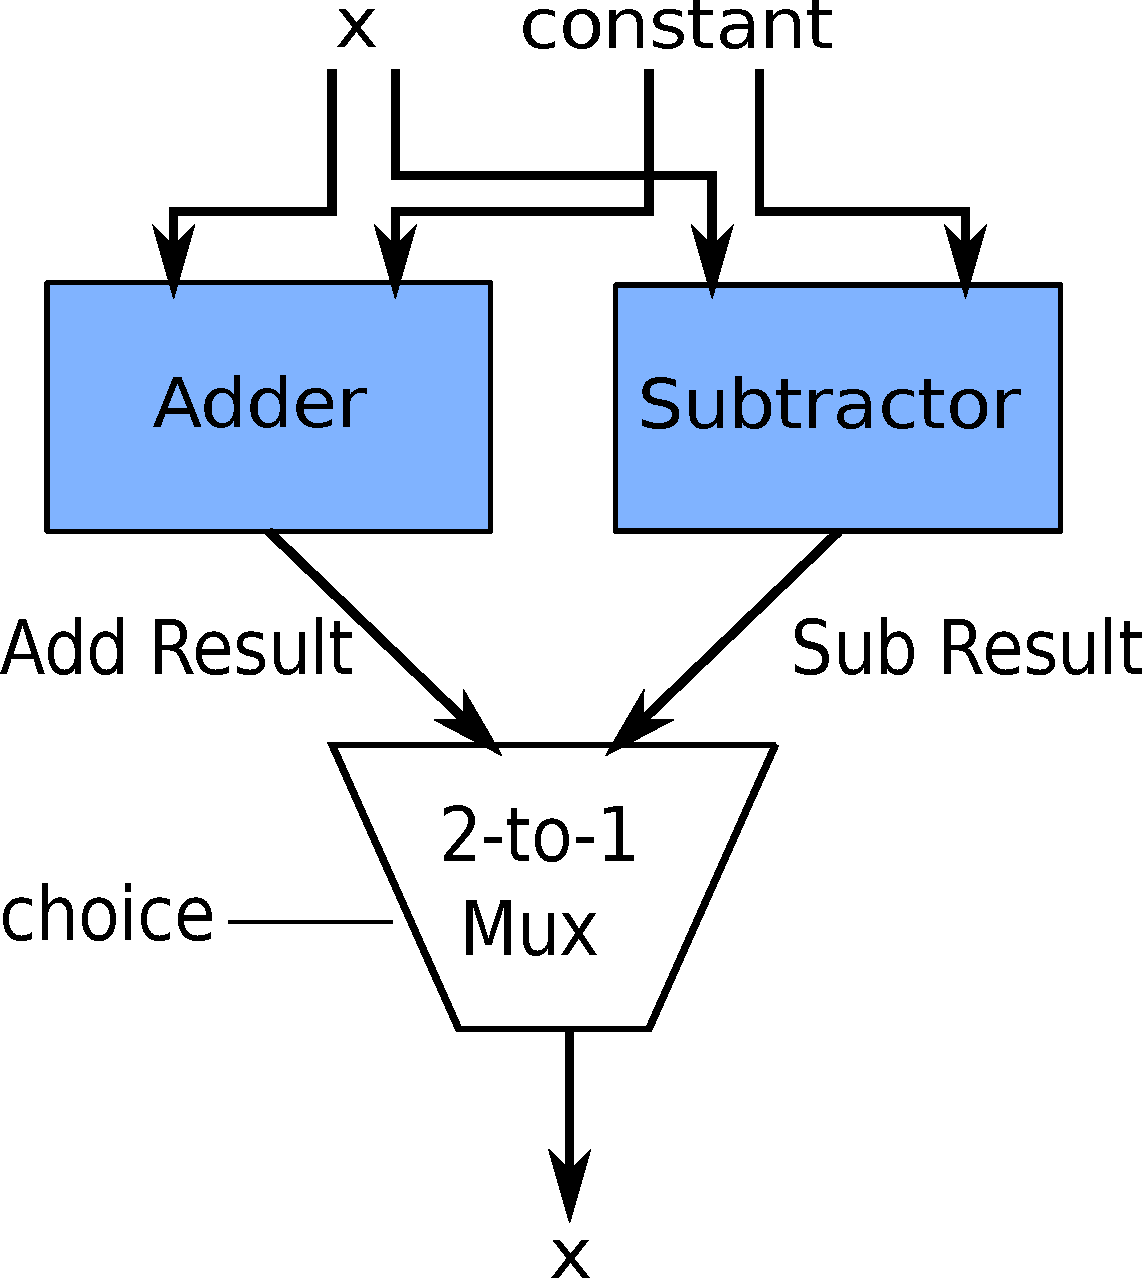
\includegraphics[width=0.5\textwidth]{domino_circuit.pdf}
  \caption{Circuit for the atom}
  \label{fig:alu_diag}
  \end{subfigure}
  \hspace{0.1\columnwidth}
  \begin{subfigure}{0.3\columnwidth}
  \begin{lstlisting}[belowskip=-0.8 \baselineskip]
  bit choice = ??;
  int constant = ??;
  if (choice) {
    x = x + constant;
  } else {
    x = x - constant;
  }
  \end{lstlisting}
  \hspace{0.1\columnwidth}
  \caption{Atom template.}
  \label{fig:alu_in_sketch}
  \end{subfigure}
  \caption{An atom and its template. The atom above can add or subtract a
constant from a state variable {\tt x} based on two configurable parameters,
{\tt constant} and {\tt choice}. Each ``??'' in the template represents a
configuration parameter that must be instantiated so that the atom implements
some computation. For instance, setting choice to 1 and constant to 1 allows us
to implement x=x+1 using this atom.}
  \label{fig:atom}
\end{figure}
%TODO: Ensure the subfigures line up in the above figure.


\subsection{The \absmachine machine model}

A programmable router that provides programmability in parsing and match-action
processing~\cite{rmt, xpliant, flexpipe, tofino} has the architecture shown in
the top half of Figure~\ref{domino_fig:router}: a programmable parser, followed
by an ingress pipeline, followed by a scheduler, followed by an egress
pipeline.  \absmachine (the bottom half of Figure~\ref{domino_fig:router})
models the ingress or egress router pipeline.  It models the computation within
a match-action table in a stage (\ie the action half of the match-action
table), but not how packets are matched (\eg exact match or wildcard match).
\absmachine does not model packet parsing and assumes that packets arriving to
\absmachine are already parsed.

 Concretely, \absmachine is a feed-forward pipeline because it is hard to
physically route backward-flowing wires that would be required for feedback.
\absmachine consists of a number of stages executing synchronously on every
clock cycle.  Each stage processes one packet every clock cycle and hands off
one packet to the next stage every clock cycle. Note that while the throughput
of a stage is one packet per clock cycle, the latency of a packet through a
stage can be multiple clock cycles (to extract headers for a match, perform the
match, and then perform the action). This is handled by internally pipelining
each \absmachine stage (\S\ref{ss:internal_pipeline_stage}).

Unlike a CPU pipeline, which occasionally experiences pipeline stalls,
\absmachine's pipeline is deterministic, never stalls, and always sustains the
router's line rate even at the smallest packet size---and hence the highest
packet processing rate. However, relative to a CPU pipeline, \absmachine is
restricted in the operations it supports (\S\ref{s:atomConstraints}).

\subsection{Atoms: \absmachine's processing units}
\label{ss:atoms}
 An {\em atom} is an atomic unit of packet processing supported natively by a
\absmachine machine, and the atoms within a \absmachine machine form its
instruction set. Each pipeline stage in \absmachine contains a vector of atoms.
Atoms in this vector modify mutually exclusive sections of the same packet
header in parallel in every clock cycle, and process a new packet header every
clock cycle.

In addition to packet headers, atoms may modify persistent state on the router
to implement stateful data-plane algorithms. To support such algorithms at
a router's line rate, the atoms for a \absmachine machine need to be
substantially richer (Table~\ref{tab:templates}) than the simple RISC-like
stateless instruction sets for programmable routers~\cite{rmt}. We explain why
below.

Suppose we need to atomically increment a router counter to count packets. One
approach is hardware support for three simple RISC-like single-cycle
operations: (1) \textit{read} the counter from memory in the first clock cycle,
(2) \textit{add} 1 in the next, and (3) \textit{write} it to memory in the
third.  This approach, however, does not provide atomicity. To see why, suppose
packet $A$ increments the counter from 0 to 1 by executing its read, add, and
write at clock cycles 1, 2, and 3 respectively.  If packet $B$ issues its read
at time 2, it will increment the counter again from 0 to 1, when it should be
incremented to 2.

Locks over the shared counter are a potential solution.  However, locking
causes packet $B$ to wait during packet $A$'s increment, and the router no
longer provides a deterministic throughput of one packet every clock cycle. CPUs employ
micro-architectural techniques such as operand forwarding for this problem. But
these techniques still suffer pipeline stalls, which prevents line-rate
performance from being achieved under worst-case conditions. Instead,
\absmachine's approach to resolving this problem is to provide a small set of
atomic operations that complete within a clock cycle. Programs that require
multi-cycle atomic operations are rejected because line-rate performance cannot
be guaranteed for them under worst-case conditions.

For instance, in the case of the counter, \absmachine provides an atomic
increment operation with an {\em atom} to read a counter, increment it, and
write it back in a single stage within one clock cycle. It uses the same
approach of reading, modifying, and writing back to implement a limited set of
other stateful atomic operations that complete within a clock cycle.
Table~\ref{tab:templates} provides one representative set of atoms.

Unlike stateful atomic operations, stateless atomic operations are easier to
support with simple RISC-like instructions for binary operations on a pair of packet
fields.  Consider, for instance, the operation {\tt pkt.f1 = pkt.f2 + pkt.f3 -
pkt.f4}.  This operation does not modify any persistent router state and only
accesses packet fields. It can be implemented atomically by using 2 atoms in a
2-stage pipeline. In the first stage, an atom adds fields f2 and f3 and writes
the result to a temporary. In the second stage, another atom subtracts f4 from
the temporary. Generalizing from this example, an instruction set designer can
provide {\em simple} stateless instructions operating on a pair of packet
fields. These instructions can then be composed into larger stateless
operations, without designing atoms specifically for each stateless operation.

\Para{Representing atoms.}
An atom is represented by a body of sequential code that captures the atom's
behavior. It may also contain internal state local to the atom. An atom
completes execution of this entire body of code, modifying a packet and any
internal state before processing the next packet. The designer of a
programmable router would develop these atoms, and expose them to a router
compiler as the programmable router's instruction set, \eg
Table~\ref{tab:templates}.

Using this representation, a router counter that wraps around at a value of 100
can be written as the atom:\footnote{We use {\tt p.x} to represent field {\tt
x} within a packet {\tt p} and a bare {\tt x} to represent a state variable
{\tt x} that persists across packets.}
\begin{lstlisting}[style=customc, numbers=none, frame=none]
if (counter < 99)
  counter++;
else
  counter = 0;
\end{lstlisting}

Similarly, a stateless operation like setting a packet field to a constant
value can be written as the atom:
\begin{lstlisting}[style=customc, numbers=none, frame=none]
  pkt.field = value;
\end{lstlisting}

\subsection{Constraints for line-rate operation}
\label{s:atomConstraints}

\Para{Memory limitations.} State in \absmachine is local to each atom.  It can
neither be shared by atoms within a stage, nor by atoms across stages. This is
because building multi-ported memories (to store the state) accessible to
multiple atoms is technically challenging and consumes additional chip area.
However, state can be read into a packet header in one stage, for subsequent
use by a downstream stage. Figure~\ref{fig:flowlet_pipeline} shows an example:
{\tt last\_time} is read into {\tt pkt.last\_time} in stage 2, for subsequent
use by stage 3.  But, the \absmachine pipeline is feed-forward, so state can
only be carried forward, not backward.

\Para{Computational limitations.} Atoms need to execute atomically from one
packet to the next, so any state internal to the atom must be updated before
the next packet arrives.  Because packets may be separated by as little as one
clock cycle, we mandate that atom bodies finish execution within one clock
cycle, and constrain atom bodies to do so.

We constrain atom bodies by defining {\it atom templates}
(\S\ref{ss:code_gen}).  An atom template is a program with configurable
parameters that terminates within a clock cycle and specifies the atom's
behavior.  Termination within a clock cycle is enforced by ensuring that the
atom's digital circuit meets timing at a given clock rate (\S\ref{ss:targets}).
An example is an ALU with a restricted set of primitive operations
(Figure~\ref{fig:alu_diag}). Atom templates allow us to create and experiment
with \absmachine machines with different atoms. As programmable routers evolve,
we expect that atoms will evolve as well, but constrained by the clock-cycle
requirement.

\Para{Resource limits.} We also limit the number of atoms in each stage
(\textit{pipeline width}) and the number of stages in the pipeline
(\textit{pipeline depth}). This is similar to limits on the number of stages,
tables per stage, and memory per stage in programmable router
architectures~\cite{lavanya_compiler, rmt}.

\subsection{Limitations of \absmachine}
\label{domino_ss:limitations}

\absmachine is a good fit for data-plane algorithms that modify a small set of
packet headers and carry out small amounts of computation per packet.
Data-plane algorithms like deep packet inspection and WAN optimization require
a router to parse and process the packet payload as well, effectively parsing a
large ``header'' consisting of each byte in the payload. This is challenging to
implement on a router that processes packets at 1 GHz, and such algorithms are best left to
general-purpose, but slower, CPUs~\cite{e2}.  Some
algorithms require complex computations, but not on every packet, \eg a
measurement algorithm that periodically scans a large table to perform garbage
collection.  \absmachine's atoms model small operations that occur on every
packet, and are unsuitable for such complex operations that span many clock
cycles.
